\documentclass[bachelor,lith,showtrims,english]{liuthesis}
\setcounter{secnumdepth}{4}
\setcounter{tocdepth}{4} 
%% Settings go in settings.tex
\PassOptionsToPackage{maxbibnames=99}{biblatex}
%%% settings.tex --- 
%% 
%% Filename: settings.tex
%% Description: 
%% Author: Ola Leifler
%% Maintainer: 
%% Created: Tue Oct 19 21:11:31 2010 (CEST)
%% Version: $Id$
%% Version: 
%% Last-Updated: Tue Dec  1 15:35:51 2015 (+0100)
%%           By: Ola Leifler
%%     Update #: 39
%% URL: 
%% Keywords: 
%% Compatibility: 
%% 
%%%%%%%%%%%%%%%%%%%%%%%%%%%%%%%%%%%%%%%%%%%%%%%%%%%%%%%%%%%%%%%%%%%%%%
%% 
%%% Commentary: 
%% 
%% 
%% 
%%%%%%%%%%%%%%%%%%%%%%%%%%%%%%%%%%%%%%%%%%%%%%%%%%%%%%%%%%%%%%%%%%%%%%
%% 
%%% Change log:
%% 
%% 
%% RCS $Log$
%%%%%%%%%%%%%%%%%%%%%%%%%%%%%%%%%%%%%%%%%%%%%%%%%%%%%%%%%%%%%%%%%%%%%%
%% 
%%% Code:

\usepackage[backend=biber,hyperref]{biblatex}
%% To set the font of your thesis, use the \setmainfont{} command,
%% surrounded with \ifxetex if you want to switch between xelatex and pdflatex
\ifxetex 
\setmainfont [Scale=1.2]{Optima}
\fi

%%%%%%%%%%%%
%% The VZ43 chapter style, from Memoir contributed chapter styles: ftp://ftp.tex.ac.uk/ctan%3A/info/MemoirChapStyles/MemoirChapStyles.pdf
%%%%%%%%%%%

\usepackage{calc,color}
\newif\ifNoChapNumber
\newcommand\Vlines{%
\def\VL{\rule[-2cm]{1pt}{5cm}\hspace{1mm}\relax}
\VL\VL\VL\VL\VL\VL\VL}
\makeatletter
\setlength\midchapskip{0pt}
\makechapterstyle{VZ43}{
\renewcommand\chapternamenum{}
\renewcommand\printchaptername{}
\renewcommand\printchapternum{}

\renewcommand\chapnumfont{\Huge\bfseries\centering}
\renewcommand\chaptitlefont{\Huge\bfseries\raggedright}
\renewcommand\printchaptertitle[1]{%
\Vlines\hspace*{-2em}%
\begin{tabular}{@{}p{1cm} p{\textwidth-3cm}}%
\ifNoChapNumber\relax\else%
\colorbox{black}{\color{white}%
\makebox[.8cm]{\chapnumfont\strut \thechapter}}
\fi
& \chaptitlefont ##1
\end{tabular}
\NoChapNumberfalse
}
\renewcommand\printchapternonum{\NoChapNumbertrue}
}
\makeatother


%% To set bibliography options, refer to the biblatex manual and use
%% the ExecuteBibliographyOptions command below to set your options

% \ExecuteBibliographyOptions{}


%% Change this to your appropriate BibTeX reference file (.bib)

\addbibresource{references.bib}

%%%%%%%%%%%%%%%%%%%%%%%%%%%%%%%%%%%%%%%%%%%%%%%%%%%%%%%%%%%%%%%%%%%%%%
%%% settings.tex ends here

%%% Local Variables: 
%%% mode: latex
%%% TeX-master: "demothesis"
%%% End: 

\usepackage{rotating}
\usepackage{color}
\usepackage{float}
\usepackage{subcaption}
\usepackage{caption}
\usepackage{graphicx}
% \usepackage{changebar}

\department{Institutionen för datavetenskap}
\departmentenglish{Department of Computer science}
\departmentshort{IDA}
\supervisor{Niklas Carlsson and Vengatanathan Krishnamoorthi}
\examiner{Nahid Shahmehri}
\titleenglish{Geo-based media player}
\titleswedish{Geobaserad mediaspelare}
\subtitleenglish{An interactive interface for geo-based video streaming}
\thesissubject{Datateknik}

\publicationyear{16}
\currentyearthesisnumber{001}
\dateofpublication{2016-06-20}


%\author{\texttt{\textbackslash author}}
\author{Andreas Nordberg\\Jonathan Sjölund}

\begin{document}

\chapterstyle{VZ43}

\chapter{Introduction}
\label{cha:introduction}

Streaming has evolved and become more popular over the last couple of years. Thousands upon thousands of different streams are being watched every day\footnote{Twitch statistics https://stats.twitchapps.com/, Fetched: 2016-04-01}, thus the demand for better and more ways to stream and view streams are longed for. If we could stream videos in different ways we can create a more interesting streaming environment, this can provide both better entertainment but also a better way to potentially improve observation in science and other areas more reliably. If a stream can provide the possibility for watching a video from different angles it can give people the option to observe and also enjoy something from different perspectives. This project focuses on accomplishing this, by creating a geo-based video player that uses HTTP-adaptive streaming (HAS) which allows for users to view a video from different angles and change between them seamlessly without any buffering delay or stuttering. By looking at an existing video streaming player and improving it to accomplish this task, we show that it's a feature worth implementing in already existing media players.

In this project we design and develop a geo-based command-and-control video streaming player using geo-tags. In practice this is a service in which you can choose between a set of recording streams of the same event, for example, but slightly different locations and angles. This would be a useful feature to have in any larger event where you would want to show the same scene from different locations and angles. The interface should then be able to automatically accept multiple coordinates for these streams and draw them in this graphical interface. The interface will be useful for both event-organizers that hire staff to make several different recordings of the same scene for on-demand viewing, but could also be used by the public who volunteer to record the event live. One major thing this interface also could be used for is during a disaster event or something of the sort, by helping the police, medical or the emergency service by allowing them to view a disaster scenario from multiple angles to help them in their communication. In such a scenario, being able to swap between different video streams would give them a better understanding of the scenario and what needs to be done in their work.

\section{Boundaries}
\label{sec:boundaries}

The application we provide is only going to be a proof-of-concept, which means we will only focus on the functionality of the video player. Factors like a designing a pretty interface and a more extensive focus on user friendliness on broader spectrum will be neglected. We will focus on making the application work for only one user to verify the functionality we want to accomplish. The number of video streams that we will initially be able to switch between will, for the purpose of testing, be limited to a few but then expanded upon to support any reasonable number of streams. This is because our main focus is to make sure that it is possible to switch between video streams, not that it's possible to do so with a large number of streams. The reason for this is that pre-buffering many videos can be difficult to accomplish with a large number of video streams and it can come with a trade-off of bandwidth usage \cite{watchingprefetching} and less efficient bandwidth usage when downloading in parallel \cite{scalableOnDemand}. As long as we provide a way to make it function for a few amount of streams the solution can be expanded upon afterwards.
\chapter{Background and Related Work}
\label{cha:theory}

To be able to grasp the concept of how HTTP-adaptive streaming (HAS) and geo-based streaming (GBS) works, a background is presented on HAS and GBS. Since the use of HAS and GBS is essential, when programming the functionalities of the interface, there is a need to study existing and related works. In this chapter studies about HAS, non-linear streaming and multipath will be presented. There will also be information about the media player that is used. This knowledge is important to be able to implement a generalized media player that allow adaptive streaming with seamless switching between videos from different geographical positions. Studies about branching videos will also be discussed since it is something that this projects builds upon.

\section{HTTP-based Adaptive Streaming}
\label{sec:has}

Mobile users streaming media sometimes suffer from playback interruptions when faced with a bad wireless connection. HTTP-adaptive streaming (HAS) seeks to resolve this by dynamically changing the bitrate, and therefore also the quality of the stream, to make do with the connection that is available to the user. To ensure smooth transitions between these quality changes HAS also tries to predict the download rates and best quality changes in advance using various methods depending on the HAS framework. There are many algorithms for these predictions and there also some works that have evaluated these kind of HAS algorithms \cite{experimentalevaluation,hastohelp}. A brief example of an algorithm would be to use previous logged connectivity history and future connectivity using geo-based methods to make predictions. With these HAS predictions, a stream quality fitting the user’s network quality can be buffered \cite{gtube}.

When implementing HAS into the geo-based interface there is a need to prefetch data from several close-by video streams at the recording area (if not all, depending on number of them) and build up a small enough buffer that makes switching between these different streams seamless. By looking at how HAS is used when implementing an interactive branched video we can say that parallel TCP connections are a must in-order to achieve this with the cost of wasting bandwidth and lower playback quality. This depends mainly on the number of videos that needs to be prefetched. Most HAS video players has a cap on the buffer size in order to avoid wasting bandwidth. 

Krishnamoorthi et al. \cite{qualbranch} use a customized HAS player that solves the problem of tradeoff between quality and number of chunks downloaded. The playback chunks are stored in the playback buffer while the prefetched chunks are stored in a browser cache, thus allowing those chunks to be retrieved quickly. This ensures that no playback interruption occurs for the user. The way they download the chunks are done in a round-robin way to ensure that a buffer workahead is built up enough for seamless playback in parallel TCP downloading. When estimating download rate of available bandwidth most HAS players often uses weighted average of past download time/rates \cite{qualbranch}. 

As argued by Carlsson et al. \cite{optimizedstreaming}, downloading chunks in a round-robin way is also a good approach for our context with parallel streaming. In our media player, this method will be used together with the idea of prefetching in the downtime of a HAS-player. Most HAS-players has some kind of buffer treshold $T_{max}$ where downloading is interrupted when reached and will resume only when the minimum buffer $T_{min}$ is reached. This kind of behaviour can be called an \textit{on-off behaviour} which can lead to poor performance under conditions with competing traffic \cite{bandawarePrefetch,whathappens}. It is common in several HAS-players like Netflix and Microsoft Smooth Streaming for example \cite{bandawarePrefetch}. 

Krishnamoorthi et al. \cite{bandawarePrefetch} provide policies and ideas that reduce the start-up time of videos by an order of magnitude and ensures the highest possible playback quality to be viewed. These policies provide a way of improving channel utilization which allows for instantaneous playback of prefetched videos without playback quality degradation. A HAS solution is suggested which we want to take advantage of together with prefetching nearby streams in a round-robin way. The solution allows for prefetching and buffer management in such a way that videos can be downloaded in parallel and switched to instantaneously without interrupting the user experience. By using a novel system to utilize the unused bandwidth during off-periods this allows for videos to simultaneously be prefetched while maintaining a fair bandwidth share. It also increases the playback quality in which a video is downloaded \cite{bandawarePrefetch}. This idea will be discussed further in \textit{Section} \ref{sec:prefetching} when we describe our idea of downloading streams.

There are some other works that have looked at optimiziation of video quality by observing and controlling the playback buffer by in turn looking at the network capacity, providing an algorithm for optimizing the video quality without any unnecessary buffering \cite{bufferbased}.

%There are works that talks about policies for providing a good way of prefetching several videos in different ways, providing means of allowing prefetching and instantaneous playback without playback quality degradation. The work studies the off-periods observed in HAS-players to utilize it as effectively as possible \cite{bandawarePrefetch}. 

There can occur several problems in HAS players \cite{qualbranch}. Huang et al. \cite{streamrate} show that when a competing TCP flow starts, a so called “downward spiral effect” occurs and the downgrade in throughput and playback rate becomes severe. This is caused by a timeout in the TCP congestion window, high packet loss in competing flows and when a client has a low throughput. The playback rate is then lower due to smaller buffer segments which makes a video flow more susceptible to perceiving lower throughput and thus creating a spiral. A possible solution is to have larger segment sizes and by having an algorithm which is less conservative, meaning that a video is requested at lower rate than it's perceived. This is something to keep in mind since quality can decrease drastically when having several videos buffering in parallel, though we will not have to buffer a full video at the same time but only chunks of a video while the main stream is being watched.

Figures \ref{fig:HAS1} and \ref{fig:HAS2} illustrate an example of a stream consisting of chunks being played, how these chunks are prefetched and stored and a swap between two streams.

\begin{figure}[!ht]
\begin{center}
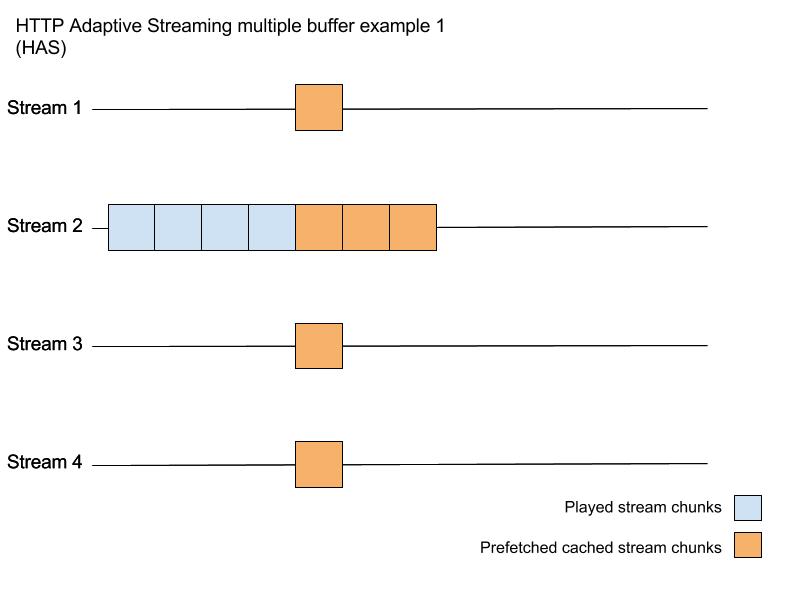
\includegraphics[scale=0.4]{HAS1.png}
\caption{HAS Parallell Stream Buffer 1}
\label{fig:HAS1}
\end{center}
\end{figure}

\begin{figure}[!ht]
\begin{center}
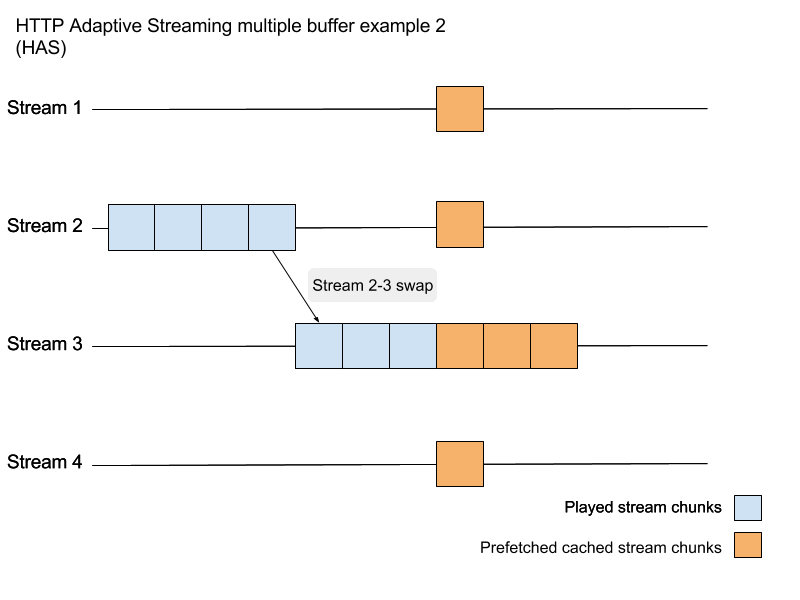
\includegraphics[scale=0.4]{HAS2.png}
\caption{HAS Parallell Stream Buffer 2}
\label{fig:HAS2}
\end{center}
\end{figure}

\section{Non-linear Streaming and Multipath}
\label{sec:nonlinear}
There are many related works which discuss non-linear streaming and multipath \cite{qualbranch, hasmultipath,scalableOnDemand,optimizedbroadcast}. Many of these works are focusing on branching videos in media players, which describes ways to allow for users to seamlessly switch between videos without quality degradation or interruptions \cite{qualbranch, hasmultipath,scalableOnDemand}. Krishnamoorthi et al. \cite{hasmultipath} presents optimized prefetching and techniques for managing prefetched chunks in a playback buffer. Prefetching from different branches to allow seamless switching between videos, using the notion of multipath non-linear videos to stitch together videos using a novel buffer management and prefetching policy. This prefetching decreases the time it takes to switch between branches considerably and is something we will take advantage of since the code we use from Krishnamoorthi et al. \cite{qualbranch} is based on a similar policy as in this project work \cite{hasmultipath}. 

If we look at what Zhao et al. \cite{scalableOnDemand} wrote they describe how choosing a correct branching point sufficiently ahead of time with an accuracy of 75 \% greatly reduces bandwidth requirements, by requesting non-linear video content where chunks are downloaded in parallel without causing jitter. This is something which is really efficient and important for users that would like the ability to switch between different videos on-demand. Selecting what type of chunks should be downloaded is hard to accomplish, at least on a broader context when considering watching TV-streams during TV-broadcasting. Zhao et al. \cite{scalableOnDemand} propose protocols that enables the possibility of scaleable on-demand content with minimal server load and developing a way that limits the lower bound bandwidth requirement using multicast \cite{scalableOnDemand}. 

%D.Gotz \cite{scalableadaptivestreaming} present a framework called Channel Set Adaptation (CSA) which allows for efficient non-linear streaming of datasets to large groups over a wide range of operating conditions. By looking at how system performance changes for an increasingly larger and larger group with unicast, broadcast and multicast he found that CSA works best for large groups when using broadcasting. He show scalable and adaptive streaming for non-linear media, achieving scalability by removing all per-client work from the server. Each client handles their own adaptive tasks through management of a set of active communications channels.

There have been works that have looked at a way of optimizing periodic broadcast delivery for non-linear media, by creating functions and algorithms that provides a way to effectively control quality of service for clients with varying playback paths. They look at cases where clients makes a path selection at their arrival instance over branching tree paths and graphs and show that the start-up delay increases exponentialy with the number of branching paths and that linear increase in bandwidth decrease the start-up delay exponentialy \cite{optimizedbroadcast}.

Many related works are mostly focused on branching videos which is simliar but not entirely similar to what is done in this project \cite{qualbranch, hasmultipath,scalableOnDemand}. This thesis will contribute more to the possibility of prefetching several videos in parallel and then be able to switch to any of them on-demand. However, the ideas used when handling branching videos is something that will be used in the geo-based media player.

\section{Strobe Media Playback}
\label{sec:smp}

To display the stream in our application we will be using a media player called Strobe Media Playback (SMP), created with the Open Source Media Framework (OSMF) by Adobe Systems. The OSMF itself is build upon Adobe Flash Player. While becoming more outdated by the day, and discontinued by some, it is still widely used for media and other graphic applications and suffices to use for the proof-of-concept of our application. In practice, this means that the media player is created using the tools that OSMF provides, compiled into a runnable flash file byte code and run by Adobe Flash Player. OSMF supports a number of important features that will be used within geo-map interface. Most importantly it enables the use of HAS with its HTTP-streaming support and progressive downloading. It also enables the player to seamlessly switch between several media elements by using a composition of “nested serial elements”, which will be prominently used within the developed application \cite{osmf}.


\chapter{System Design}
\label{cha:sysdesign}

To advance in this project we will mainly be programming, designing and developing the application. The programming language of choice will be Adobe ActionScript and the IDE Flash Builder, which is very similar to the IDE Eclipse. The interface to be developed should have multiple functionalities. We want the interface to accept incoming video streams tagged with a location and cardinal direction from expected sources. The video streams will have to be tagged with these geographical data, which is not a common included feature with most video recording softwares. Developing a separate recording application to create these kind of geo-tagged video streams, for the sake of this project, is outside of the scope of the thesis. Instead, we will prove the functionality of our interface with synthetically generated video geo-tags. These streams will then be made to work with the custom OSMF player.  Under-the-hood features will include HAS to ensure a smooth playback of the streams, both for buffering a single stream but also for prefetching and buffering a fraction of the other streams to ensure uninterrupted playback during stream swaps. To help us focus on the main problem of developing this interface, we are being provided with some existing code by our supervisors. This includes a working SMP player created with a modified version of OSMF with code from an existing HAS-interface using prefetching \cite{qualbranch}.

\section{Interface Design}
\label{sec:interfacedesign}

The main part of this project is to expand upon the existing user interface (UI) of the default SMP player, as seen in Figure \ref{fig:mediaplayer}, and create a new section of it where we can implement the new desired functionality of this project. 

\begin{figure}[ht!]
\begin{center}
	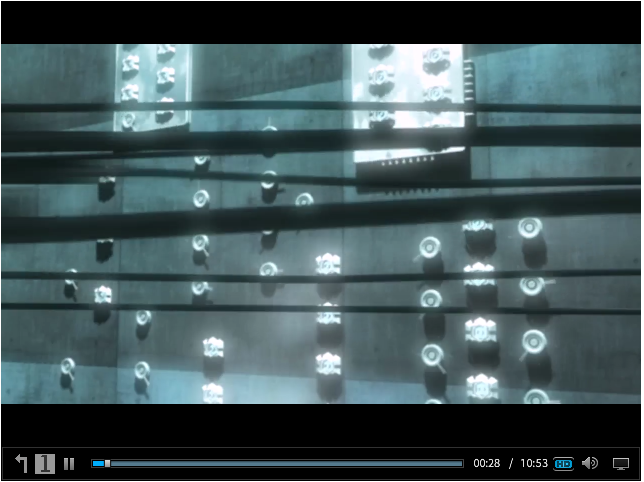
\includegraphics[scale=0.7]{Media_player.png}
	\caption{Strobe Media Player}
	\label{fig:mediaplayer}
\end{center}
\end{figure}

\begin{figure}[ht!]
\begin{center}
	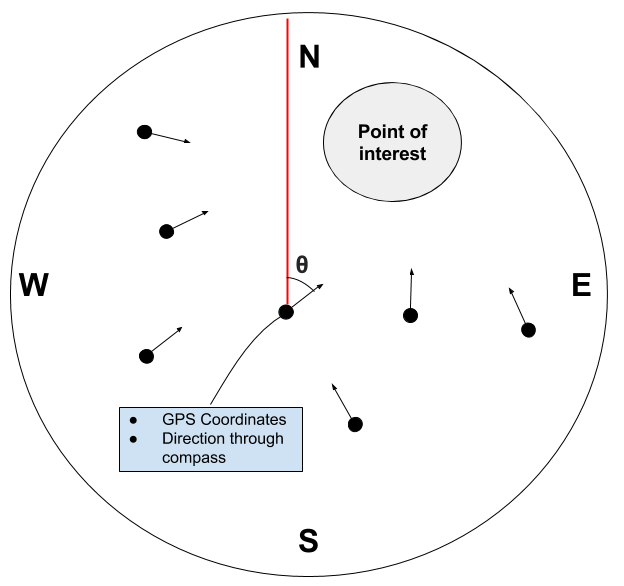
\includegraphics[scale=0.6]{teomet.png}
	\caption{Conceptual interface of GPS and Direction selection map}
	\label{fig:gpsinterface}
\end{center}
\end{figure}

For our interface design we decided to add an additional button to the control bar of the UI. When pressed, a graphical interface similar to the one in Figure \ref{fig:gpsinterface} is shown in the media player. Within this graphical interface, the user can hover over the arrows representing the available video streams located at different geographical locations and angles in the area. While hovering over an arrow a tool-tip is shown with information about the video in question, including the GPS-coordinates and the angle, providing the user with a comprehensive overview of the available stream. Finally, when an arrow is clicked the selected video is played.

Along with these arrow objects representing the video streams in the graphical interface, the layout will also display an optional “Point of interest” with its own geographical position. This point of interest is usually the center of attention of all the different video streams and can be the main attraction of anything from a concert to some other large event. The implemented geographical view will also display the north, west, east and south cardinal directions to know the angle of the every stream relative to them. The angle $\theta$ in Figure \ref{fig:gpsinterface} is taken from the magnetic heading from a recording client, which is the direction relative to north that the client interprets. This will give us the direction relative to the north cardinal direction.

\section{Prefetching Principle}
\label{sec:prefetching}

As mentioned briefly in \textit{Section} \ref{sec:has}, chunks will be downloaded in a round-robin way and chunks will be downloaded only during the downtime of the HAS-player. Krishnamoorthi et al. \cite{bandawarePrefetch} mention a policy called \textit{best-effort} that we will use, in which chunks from other videos are only downloaded after the buffer size has reached $T_{max}$ and will not until then start to prefetch chunks from several other videos. These chunks are only going to download as long as the buffertreshhold does not go below $T_{min}$ for the currently streamed video. The policy adapts to the available bandwidth and varying network conditions. It is also one of the better policies discussed since it downloads chunks of as many videos as possible which is an important and needed functionality in scenarios with many different streams \cite{bandawarePrefetch}. In Figure \ref{fig:prefetch} an idea of this can be seen. Other nearby streaming videos will only be downloaded once $T_{max}$ is reached. A nearby video will be prefetched only in a few chunks and the videos are downloaded in a round-robin way. Alternative video 1 followed by 2 and so on. Once the $T_{min}$ is reached the main video resumes its downloading. One idea that would be best, but will not be implemented, is what video should be prefetched first, or if it should be chosen. Prefetching distant videos may be a better choice because they are probably more likely to be switched to. An interesting idea but not considered for our proof-of-concept interface. Carlsson et al. \cite{optimizedstreaming} has also designed and implemented optimized policies for this context. Interesting future work will incorporate these policies with our geo-based interface.

\begin{figure}[ht!]
\begin{center}
	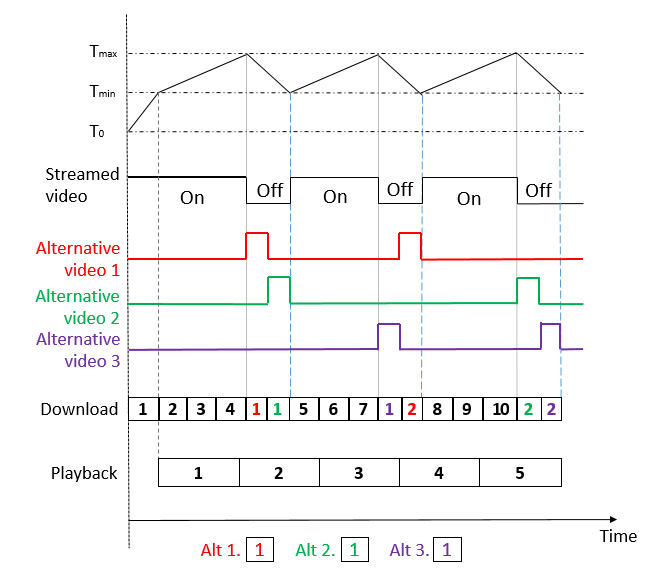
\includegraphics[scale=0.6]{prefetch.png}
	\caption{Prefetching overview}
	\label{fig:prefetch}
\end{center}
\end{figure}

\section{Server Integration}
\label{sec:serverintegration}

The SMP player is by default set to play a stream of video located at a server supporting HTTP-streaming. For this project we use the Adobe Media Server 5 for enabling the chunked video streaming needed for our HAS functionality. Since we use a similar OSMF player that were used by Krishnamoorthi et al. \cite{hasmultipath}, the quality of our prefetched chunks will be adaptive to the available bandwidth\cite{hasmultipath}.

\section{Relative Placement of Geographical Points}
\label{sec:relativeplacement}

The interface accepts an arbitrary number of video streams coupled with a cardinal direction and GPS-coordinates, including latitude and longitude values. The graphical points representing these video streams should then be placed and scaled relatively to each other on the interface's geographical map, as shown in Figure \ref{fig:gpsinterface}. To accomplish this automatic placement and scaling, an algorithm was developed to calculate where the objects should be drawn to keep their relative positions between each other, so that the graphical points accurately represents the real life locations of the recordings.

\subsection{Geographical Position Algorithm}
\label{sec:geoalgorithm}

The algorithm works as follows. First, every streamer and point of interest is an object in a list. Second, the center for which all objects will be placed relative to is calculated from all the objects. This is done by checking each and every objects latitude and longitude position and take the maximum and minimum value from them as follows:

\begin{align}
\label{eq:maxandmin}
maxX &= max\{longitude_i\},  \\
minX &= min\{longitude_i\}. \nonumber
\end{align}
 
We go through every object and take and biggest and smallest longitude value. This is done similarly for \textit{maxY} and \textit{minY} but with latitude instead of longitude. When we have the maximum and minimum value of longitude and latitude the algorithm will calculate the center of the real world map's longitude-axis and latitude-axis as follows:

\begin{align}
\label{eq:center}
centerX &= \frac{maxX+minX}{2},  \\
centerY &= \frac{maxY+minY}{2}. \nonumber
\end{align}

The formula calculates the center point of all the points for the real world map where all the points will be placed relative to. Note that \textit{centerX}, \textit{maxX} and \textit{minX} is actually spherical longitude values, similar with \textit{centerY}, \textit{maxY} and \textit{minY} which is latitude values, and not flat surface x- and y-axis values. This direct translation may cause some inaccuracy. By taking half of maximum and minimum with both longitude and latitude we can get our center point as a representation of the real world map.
 
Third, when we have the center point of all points we can calculate the maximum radius that everything will scale with as follows:

\begin{align}
\label{eq:radius}
maxRadius &= max[\frac{maxX-minX}{2}, \frac{maxY-minY}{2}].
\end{align}

The calculation checks what the maximum difference is between maximum and minimum for longitude and for latitude then takes that value as its \textit{maxRadius}. This is to get the correct radius for scaling and relativity.

Fourth, with the maximum radius calculated we can now place all the objects onto the geographical map. This is done by calculating each objects relative position to the center point that we calculated in equation \ref{eq:center} and translate it to x- and y-coordinates. This translation is done with the equirectangular approximation formula \cite{equi}:

\begin{align}
\label{eq:equiretangular}
deltaX &= (centerX-longitude_i)\cdot\frac{40000}{360} \\
 &\phantom{b=\,} \cdot cos((latitude_i+centerY) \cdot \frac{\pi}{360}), \nonumber\\
deltaY &= (latitude_i-centerY)\cdot\frac{40000}{360}. \nonumber
\end{align}

Here, \textit{deltaX} and \textit{deltaY} are the projected real world x- and y-distances between a coordinate and the center point with <$longitude_i$, $latitude_i$> and <\textit{centerX}, \textit{centerY}>. This method simply calculates the distance between two geographical points on the surface of a spherical area \cite{equi}. The translation is done to fit our geographical map as it represents a view on a flat plane. In the formula we approximate the earth's circumference as 40000 km. If we had used latitude and longitude as plain \textit{x} and \textit{y} values instead the positions would not have provided a good enough accuracy to the flat x-/y-plane because of the spherical nature of latitude and longitude coordinates. An alternative method of calculating the distance between two objects would have been the Haversine formula, which excels at accuracy along high distances \cite{haversine}. However, for smaller distances, as used in our project, equirectangular projection suffices.

With \textit{deltaX}, \textit{deltaY} and \textit{maxRadius} the relative distance on the display can be calculated. For calculating these relative distances, \textit{relX} and \textit{relY}, 
we first have to calculate a point's distance to the center point. For this, Pythagoras theorem is used:

\begin{align*}
deltaZ = \sqrt{deltaX^2 + deltaY^2}.
\end{align*}

With \textit{deltaZ} the relative placement for the point in the x- and y-axis compared to this distance can be calculated:

\begin{align}
\label{eq:percent}
percentOfX = \frac{deltaX}{deltaZ}, \\
percentOfY = \frac{deltaY}{deltaZ}. \nonumber
\end{align}

The two values,  \textit{percentOfX} and \textit{percentOfY},  represents how many percent of \textit{deltaZ} a point is placed in the x- and y-axis. With this the only thing left to do is to calculate a scaling factor, in order to rescale the point's position according to the interface's size without losing relativity: 

\begin{align*}
\gamma = \frac{deltaZ}{maxRadius*\frac{40000}{360}}.
\end{align*}

The scaling factor \textit{$\gamma$} is calculated by multiplying the \textit{maxRadius} with a constant that is used in the equirectangular formula to get the radius for x- and y-coordinates. Then we calculate how many percent of \textit{maxRadius} the distance \textit{deltaZ} is. With the scaling factor \textit{$\gamma$} a new \textit{deltaZ} can be calculated that is adapted to the interface's size:

\begin{align*}
relZ = \gamma \cdot Mapradius.
\end{align*}

The value \textit{relZ} is the distance from the interface center point and where the point should be on the interface, and \textit{Mapradius} is the radius for the interface. To calculate how much to move the point in the x- and y-axis we only need to multiply \textit{relZ} with the percent we got from equation \ref{eq:percent}:

\begin{align*}
relX = relZ \cdot percentOfX, \\
relY = relZ \cdot perecntOfY.
\end{align*}

What we basically have done is to make sure that scaling of the distances is adapted to our geographical map's boundaries. When we have the move values, \textit{relX} and \textit{relY}, the algorithm will move each object with that value from the center of the geo-map which all objects will have as its starting position. 

When executing this algorithm for geographical object placement two checks are done on all the objects to be placed. One time for equation \ref{eq:center} and one time for equation \ref{eq:equiretangular}. Since the number of objects is \textit{n} and we go through them two times the time to execute the algorithm is $\mathcal{O}(2n)$. The constant two can be removed due to the nature of big O making the final time complexity for the algorithm $\mathcal{O}(n)$.



\subsection{Simplification of the Algorithm}
\label{sec:limacc}

The geographical position algorithm places every object very good compared to reality in a way that relativity is kept. However, the equirectangular approximation formula that is used in equation \ref{eq:equiretangular} can be approximated. Since every object is placed with a relatively small distance between each other the algorithm can be simplified to the following: 

\begin{align*}
deltaX &= (centerX-longitude_i)\cdot\frac{40000}{360}, \\
deltaY &= (latitude_i-centerY)\cdot\frac{40000}{360}. \\
\end{align*}

The equation above is simpler and removes the \textit{cos} that was used previously because for small distances the value of \textit{cos} will be close to one. Since video streams in a real-life scenario will be very close when streaming the same point of interest the simplification does not cause any problems in relativity. The accuracy of the algorithm will be demonstrated in \textit{Chapter 4}.

\section{Technical Details}
\label{sec:technicaldetails}

To be able to accomplish switching between videos and getting a functional UI there are a lot of technical details to be explained in-order to get a full understanding of how the code works. Since we used the code from Krishnamoorthi et al. \cite{qualbranch} there was first a lot to understand before we could start doing anything. The problems we had and complications we encountered will be explained \textit{Chapter 5} while the focus in this section will be on \textbf{our} code and implementations. 

Our progression can be divided into different sections which will be explained in a general detail:

\begin{enumerate}
\item Making a button to open the view.

\item Making a view appear, which displays a map with a point of interest and cardinal directions.

\item Making clickable geo-map objects appear on the displayed map.

\item Connecting each geo-map object to a video and be able to play it through a class called \textit{AdvertisementPluginInfo}.

\item Making the geo-map videos interactable.

%\item (Attempting to make the geo-map switching seamless.)This will be added to result/discussion instead.

\item Adjustments and improvements of the code and the implementation of a position algorithm. 
\end{enumerate}

The details of the code and implementation will not be explained line by line but a more general idea and overview will be given of what was done.

The first step was to make an interactive button which opens the graphical interface. Three different colored assets had to be created for how the button should look like, which was designed in photoshop. The button illustrates three arrows with a dot at each end facing a general direction. This shows that a view is opened with objects similar to those. These buttons were then added to a ShockWave Component (SWC) file which stores the assets. The assets were then given an assets id and name so they could be retrieved using these as references. A class for the button was created and was added to the control bar. The button extended \textit{ButtonWidget} where it could add the assets to a "face", a kind of state, which allowed the button to switch between the different assets when changing face. 

The second step was to make a view appear that is represented as circle to better fit with how geo-map objects will be placed. For this step a widget and sprite class was created. The geo-map widget class handles the layout of the clickable layout, the creation of the geo-map view and the handling of fullscreen. The geo-map view is placed in the middle of the stage for the player and when fullscreen is initiated the graphical interface will be moved and scaled in such a way that relativity is kept. In the geo-map sprite class the position algorithm, creation of every object and cardinal direction is handled.

In the third step a new class was created called \textit{GeoMapObject} which holds all functions of the streaming video to be shown in the media player. This class have functions to add and get the position of the geo-map object, the latitude and longitude of the real life recording position, direction, setting the video stream URL to be connected with the object etc. The geo-map object which is created in the geo-map sprite class is added to a list. This list will handle all the geo-map objects on the view and is used for when clicking on an object. Together with a function in the geo-map object class it helps to show which object is clicked on and make sure that no more than one object is highlighted at the same time.

Continuing to the fourth step, the technicalities became a bit more complicated and this is the part when the servers came into play and getting the videos to show up on the media player. More details about the server will be explained in \textit{Section} \ref{sec:server}, and also the main problems and difficulties that occurred when trying to use it. For this step each video in the geo-map objects needed to be played with a class called \textit{AdvertisementPluginInfo}, which is a class created for the purpose of playing advertisement videos in the beginning, middle or end of a video. In this stage, modifications were done to the functionality of the \textit{AdvertisementPluginInfo} class from instead of playing the video acting as an advertisement halfway through the main video, to play the video acting as an advertisement at the start of the main video stream. This allows for the switch to happen directly when the geo-map object is clicked on. However, to get this to work the class also needed to first stop the main video and signal that another video is playing. For this the main media player from the Strobe Media Playback needed to be fetched and sent in to the \textit{AdvertisementPluginInfo} class as a reference. This was solved by creating the geo-map button in the SMP class and then sending the reference which was forwarded to the geo-map objects. This way the media container and media player that the SMP intitially used could be stopped and removed. When this was done the \textit{AdvertisementPluginInfo} class could change between the different videos, as if they were multiple advertisements, which meant that only playing the advertisement videos was possible but not being able to interact with them. 

Step five, which was about getting the interaction for the videos to work, was the most difficult task of them all. Since the videos were played as an advertisement some things needed to be changed, because these advertisement videos was set to not be interactable through the user interface. The main thing here is that the media player still recognizes the non-advertisement video as the main media from the Strobe Media Playback while the geo-map interface's videos was only some advertisements on top of it. What was done to fix this was to rewire all of the graphical user interface in a way that you would be able to control the advertisements with it. In other words instead of playing, pausing and interacting with the user interface for the main video, a check is done for the controls. What this check does is that it checks if an "advertisement" is being played and if it is, then the controls will be changed to affect the advertisement instead.

In the last step adjustments and improvements was done to the code and also the implementation of the position algorithm. Here the code was adjusted and improved to make sure that the implementations which were done would not crash anything else. Here, the \textit{PointOfInterest} class was implemented to better fit the relative position algorithm. Since the algorithm uses a list of all geo-map objects there was need for \textit{PointOfInterest} to be an object that uses similar functions to the ones in the geo-map object class. 

\section{Server and Video Application}
\label{sec:server}

As previously mentioned in the report the server used is the Adobe Media Server 5 (AMS 5), which is primary used for downloading videos from cache as similar to the works described in \textit{Chapter 2}. AMS 5 is a server used for HTTP-streaming which is needed in order to use HAS. The AMS 5 uses something called an Apache server, specifically Apache 2.4, which enables a video to be called with HTTP. To stream videos with the AMS 5 there can be a need to allow the the flash player to stream a HTTP-video through the local media player\footnote{Global\:Security\:Settings\:panel: https://www.macromedia.com/support/documentation/en/\\flashplayer/help/settings$\_$manager04.html}, otherwise security errors may occur. The reason for this security error being that a call is made in the code to a plug-in which allows for sending and requesting a URL to be played.

Except for using the AMS 5 to play a video through HTTP the video also needs to be in formats of F4V or FLV which are two different video file formats commonly used for delivering videos over internet using Adobe Flash Player. Every recorded video for this thesis has been converted to FLV with FFmpeg\footnote{FFmpeg: https://ffmpeg.org/} which is a free open source software project including libraries and utilities for converting multimedia data.


\chapter{Validated Results}
\label{cha:results}

To demonstrate the geo-based media player, we went out and did some recordings to test the functionalities we designed and implemented in this thesis. We went to “Blåa havet” in front of Kårallen, located at Linköping University, where some students were promoting an upcoming event with some activities. We found that this was a suitable point of interest to record from different angles for our testing case. As we only had two cameras available at the time we made three sets of recordings consisting of two recordings each, with each set displaying the same scene from two different locations and angles at the same time. The desired outcomes of this test was to prove the accuracy of the relative placement algorithm and, within the interface, be able to swap between the recordings to view the same object at one point in time from different angles.

\section{Position Algorithm}
\label{sec:positionalgorithm}

To demonstrate the accuracy of the relative placement of geographical points in the interface, we noted the GPS-coordinates and angles at the used recording locations. We then input the coordinates into Google Maps as seen in Figure \ref{fig:googlemaps}, which is used here as a reference to prove the accuracy of our placement algorithm. We also input the same latitude and longitude values into our interface along with the angles used in the recordings to test our algorithm for a few objects. We later input another larger set of coordinates into the interface including many objects to load test the algorithm. Figure \ref{fig:GeomapVsGoogleLessThan10objects} shows the comparison between the algorithm's object placement and the Google Maps reference with the coordinates used in the test case and Figure \ref{fig:GeomapVsGoogleMoreThan10objects} shows a similar comparison in the algorithm's load test. In these figures the displayed yellow stars represents Google Maps' placement of the given coordinates while the arrow-dots represents the same respective placement of the coordinates as received from the interface.


\begin{figure}[ht!]
\begin{center}
	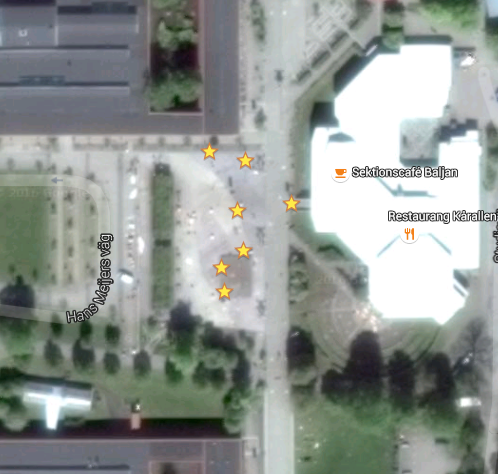
\includegraphics[scale=0.64]{Google_Maps.png}
	\caption{Google Maps view of the Streaming locations}
	\label{fig:googlemaps}
\end{center}
\end{figure}

\begin{figure}
\begin{subfigure}[b]{0.5\textwidth}
        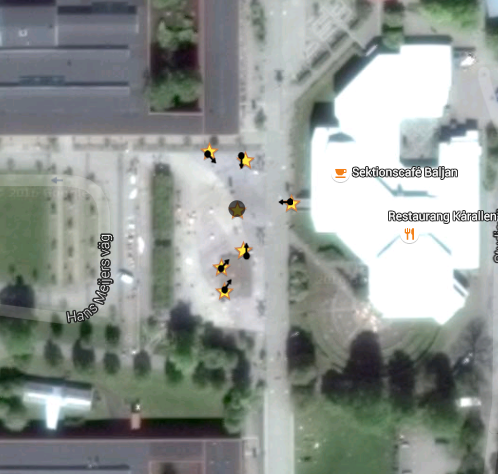
\includegraphics[width=\textwidth]{GeomapVsGooglemindrean10.png}
        \caption{Comparison with Google Maps in the test case}
        \label{fig:GeomapVsGoogleLessThan10objects}
    \end{subfigure}\hfill 
    \hspace{3px}
    \begin{subfigure}[b]{0.51\textwidth}
        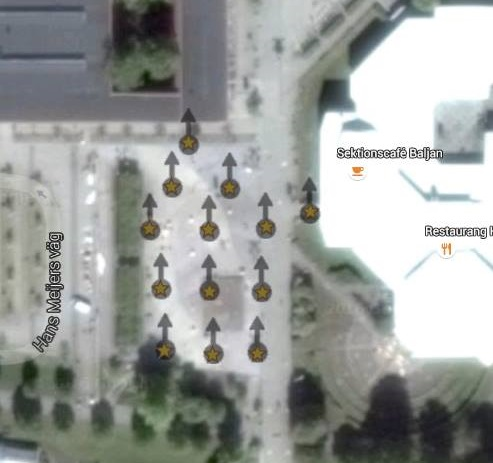
\includegraphics[width=\textwidth]{GeomapVsGooglefleran10.png}
        \caption{Comparison with Google Maps in the load test}
        \label{fig:tiger}
    \label{fig:GeomapVsGoogleMoreThan10objects}
    \end{subfigure}
	\caption{Geo-map compared to google map using equirectangular algorithm}
	\label{fig:GeomapVsGoogleWithLessThan10objects}
\end{figure}

The placement of the arrow points in Figure \ref{fig:GeomapVsGoogleLessThan10objects} is almost an exact match to the Google Maps reference stars for the respective coordinates, at least in terms off relativity. There is a slight difference between interface's placement and the reference in this figure and the reason for this is that our method for rotating the arrow points is not optimal. The default and only way of rotating a graphical object provided by our programming tools is to rotate the object around its top-left corner. Due to this we added some functionality to this existing rotation function to make the objects rotate around its center instead. Because this rotation code is not optimal there is a very slight deviation from its supposed placement. With the load test however, we did not angle the arrow points as shown in Figure \ref{fig:GeomapVsGoogleMoreThan10objects}. Because the suboptimal rotation function does not take place here the algorithm's relative placement is exactly on point with its reference.

This would prove the accuracy of our relative placement of the geographical points, albeit with a slightly better precision if the objects are not rotated. The rotation function will be further discussed in \textit{Chapter \ref{cha:discussion}}.

\section{Geo-based Streaming}
\label{sec:geobasedstreaming}

As we have mentioned before our implementations is as shown in Figure \ref{fig:gpsinterface}, where we have a button that opens the geographical map, a circle that represents a “map” and arrows pointing in a direction that represents streamers and videos. When a user selects a video the arrow is highlighted and that video is then played. In our test case, we set up two cameras at a time and did recordings of 90 seconds each. In these videos we captured many people doing various activities. There were people jumping the trampoline, using hoverboards, walking and biking around. When we input these three sets of two recordings each into our media player, we could swap between the two recordings of each set and watch these same events unfold from different positions and angles. In Figures \ref{fig:testview1A} and \ref{fig:testview2A} two different recordings are selected and they show the same event where, for example, the guy inside the red circle in the pictures are hoverboarding in front of the red shirt guy the same time of the videos. If we look at Figures \ref{fig:testview1B} and \ref{fig:testview2B} they show the geo-map interface of the views. Both interfaces shows that a different stream object is highlighted when a different view is shown. This would prove the desired functionality of where the user can display the same events unfold from different geographical positions and angles.

\begin{figure}
\begin{subfigure}[b]{0.5\textwidth}
 	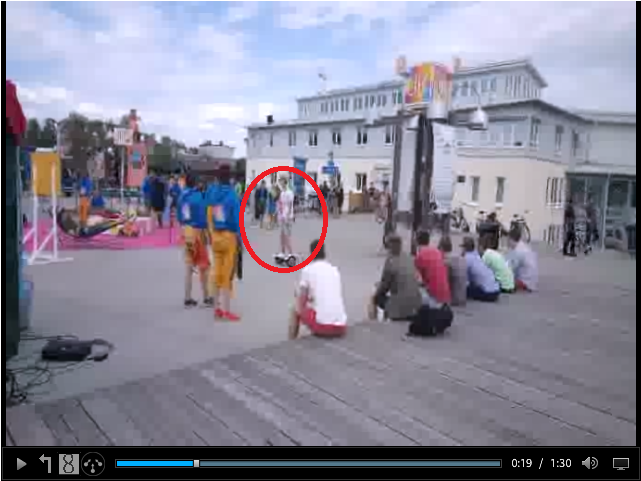
\includegraphics[width=\linewidth]{Hoverboard_1.png}
  	\caption{Test view 1 without the interface visible}\label{fig:testview1A}
    \end{subfigure}\hfill 
    \hspace{3px}
    \begin{subfigure}[b]{0.5\textwidth}
	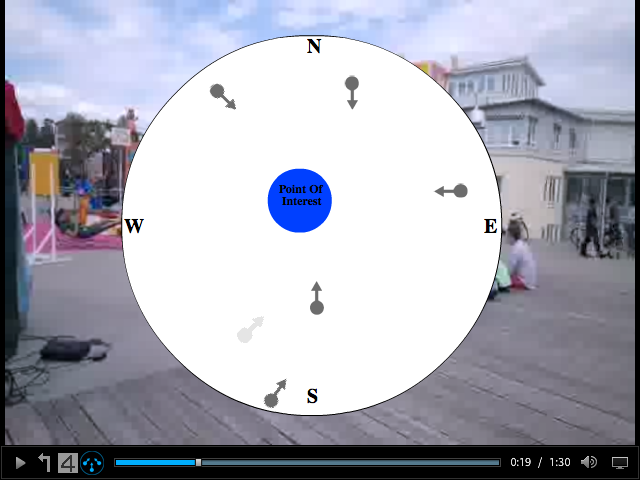
\includegraphics[width=\linewidth]{Hoverboard1medmap.png}
  	\caption{Test view 1 with the interface visible}\label{fig:testview1B}
    \end{subfigure}
	\caption{Test view 1}
	\label{fig:testview1}
\end{figure}

\begin{figure}
\begin{subfigure}[b]{0.5\textwidth}
 	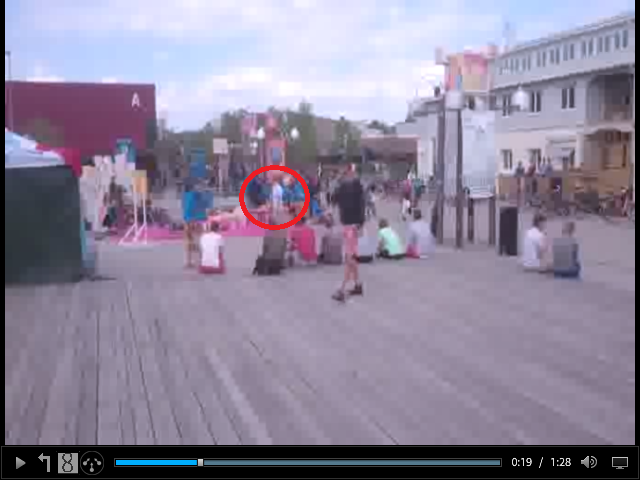
\includegraphics[width=\linewidth]{Hoverboard_2.png}
  	\caption{Test view 2 without the interface visible}\label{fig:testview2A}
    \end{subfigure}\hfill 
    \hspace{3px}
    \begin{subfigure}[b]{0.5\textwidth}
	 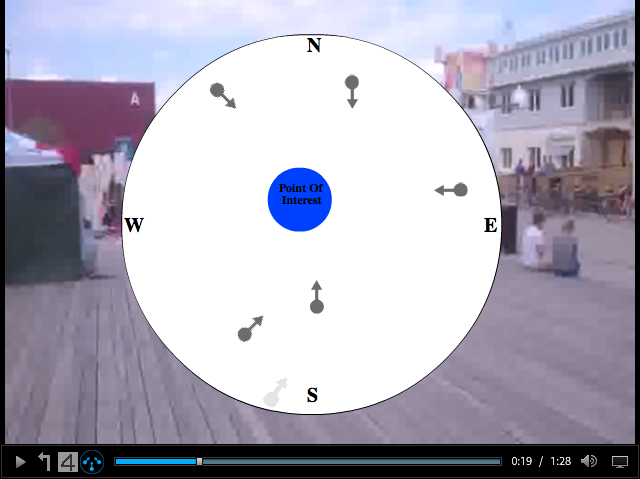
\includegraphics[width=\linewidth]{Hoverboard2medmap.png}
 	\caption{Test view 2 with the interface visible}\label{fig:testview2B}
    \end{subfigure}
	\caption{Test view 2}
	\label{fig:testview2}
\end{figure}

\section{Consistency with On-demand Switching}
Even though prefetching is not implemented we can still test the consistency of the on-demand switching, looking at the time it takes to switch between different videos on-demand. This test was done by clicking between different stream objects on the interface and measuring the time it takes from when the user clicks a stream until the stream is displayed and played in the media player. In the test we measured three different parts of this process; the time between the user clicks the stream object until the stream starts to download, the time it takes for the stream to be downloaded and ready to play and the time between this download has completed until the stream actually starts playing in the media player. Finally, we included a fourth measurement of the total time between a switch between two streams. Switching between different videos was done 200 times and four graphical representations of how long each of these processes took is shown in Figures \ref{fig:click-time} to \ref{fig:start-time}. Every part (a) of the figures represents the frequency for a certain time interval in that figure's and process’ measurement segment. Every part (b) of the figures shows the Cumulative Distribution Function (CDF) for that specific measurement, which is the probability that a certain time \textit{x} will occur.

We can see from the CDF graph in Figure \ref{fig:cdf4} that the probability that a video switch take less than 140 milliseconds is around 60 $\%$ and that the probability for a video switch under 160 milliseconds is around 83 $\%$. This means that a video switch will unlikely take more than 160 milliseconds or even more than 200 milliseconds.  The average time it took to switch is roughly 150 milliseconds, or 148 milliseconds to be precise. The median is 137 milliseconds and the standard deviation is around 37 $\%$.

The times for switching is likely a bit faster than shown in Figure \ref{fig:start-time} because of how checking the time is done. The time starts when the object is clicked and a new advertisement is created. After that a new media player is created and  the URL will be retrieved through the AMS 5. The URL will then be sent to the plug-in script and then called by the \textit{AdvertisementPluginInfo} class. The URL is then prebuffered a little bit before the video is ready to be played in which the timer will stop. The prebuffering time is shown in Figure \ref{fig:load-time}. If prebuffering of the video can be done in a more efficient way with optimized prefetching similiar to what is done in the project \cite{optimizedstreaming} the time would have been a lot faster. 

This test is done from another computer which did not host AMS 5 which means that it had to send requests of the streams to the computer hosting the AMS 5 in order to receive the videos. Keep in mind if this consistency test were done on a different performing setup with another set of computers and connections, this result would likely vary.

\hspace*{-2cm}
\begin{figure}[!ht]
\begin{subfigure}[b]{0.5\textwidth}
 	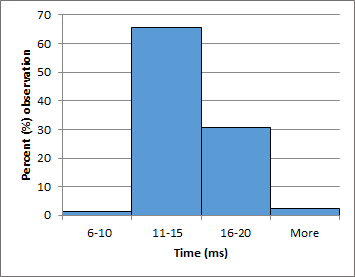
\includegraphics[width=\linewidth]{Histogram_Click-time.png}
  	\caption{Histogram}\label{fig:histogram}
    \end{subfigure}\hfill 
    \hspace{3px}
    \begin{subfigure}[b]{0.5\textwidth}
	 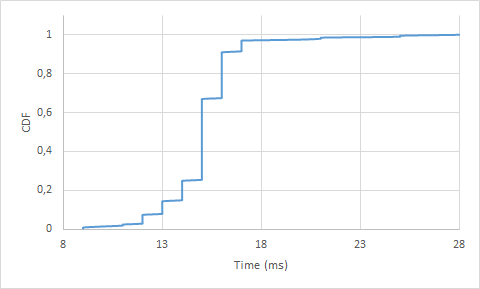
\includegraphics[width=\linewidth]{CDF_Click-time.png}
 	\caption{CDF}\label{fig:cdf}
    \end{subfigure}
	\caption{Time between click to download}
	\label{fig:click-time}
\end{figure}

\begin{figure}
\begin{subfigure}[b]{0.5\textwidth}
 	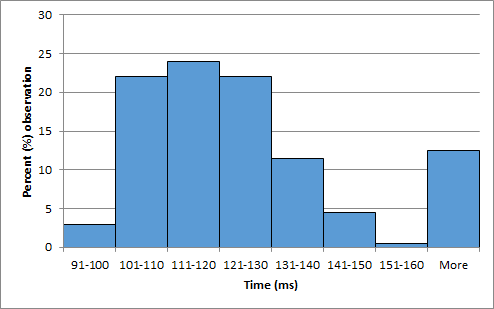
\includegraphics[width=\linewidth]{Histogram_Load-time.png}
  	\caption{Histogram}\label{fig:histogram2}
    \end{subfigure}\hfill 
    \hspace{3px}
    \begin{subfigure}[b]{0.5\textwidth}
	 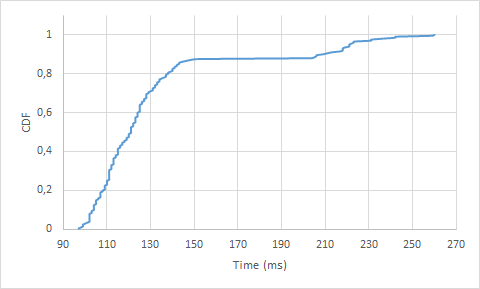
\includegraphics[width=\linewidth]{CDF_Load-time.png}
 	\caption{CDF}\label{fig:cdf2}
    \end{subfigure}
	\caption{Time to download}
	\label{fig:load-time}
\end{figure}

\begin{figure}
\begin{subfigure}[b]{0.5\textwidth}
 	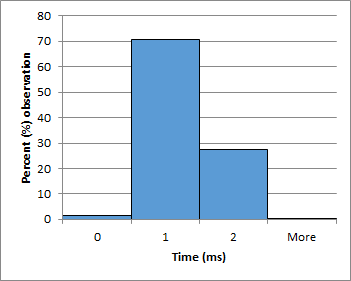
\includegraphics[width=\linewidth]{Histogram_Play-time.png}
  	\caption{Histogram}\label{fig:histogram3}
    \end{subfigure}\hfill 
    \hspace{3px}
    \begin{subfigure}[b]{0.5\textwidth}
	 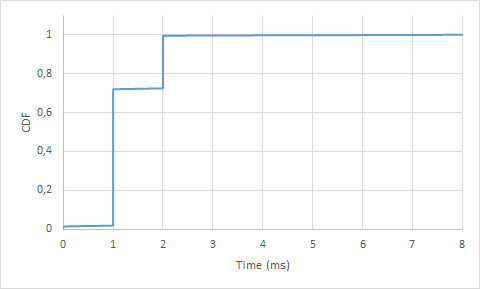
\includegraphics[width=\linewidth]{CDF_Play-time.png}
 	\caption{CDF}\label{fig:cdf3}
    \end{subfigure}
	\caption{Time between download to play}
	\label{fig:play-time}
\end{figure}

\begin{figure}
\begin{subfigure}[b]{0.5\textwidth}
 	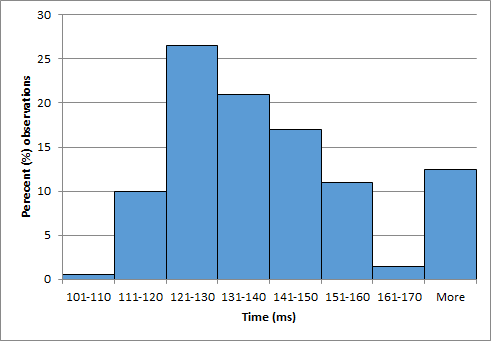
\includegraphics[width=\linewidth]{Histogram_Start-time.png}
  	\caption{Histogram}\label{fig:histogram4}
    \end{subfigure}\hfill 
    \hspace{3px}
    \begin{subfigure}[b]{0.5\textwidth}
	 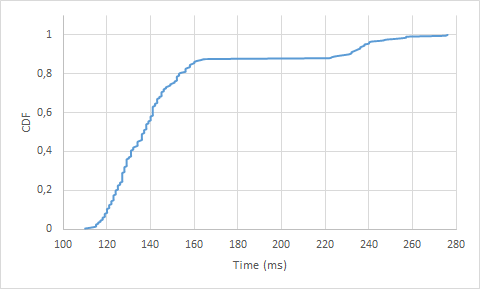
\includegraphics[width=\linewidth]{CDF_Start-time.png}
 	\caption{CDF}\label{fig:cdf4}
    \end{subfigure}
	\caption{Total time from click to play}
	\label{fig:start-time}
\end{figure}
\chapter{Discussion}
\label{cha:discussion}


During the project we faced a lot of obstacles and some things which needed to be changed. In the sections below these problems will be described, why they may have happend and how they could be fixed. What changes were made and had to be done will be discussed and also what could have been done differently.


\section{Understanding the Provided Code}
\label{sec:understandingcode}

When we started working on this assignment to make an interactive Command-and-Control center with geo-tagged streaming we first had to install and adjust to the tools given to us to develop the interface, being OSMF and SMP. These tools consisted of an extensive amount of existing code which we had to delve into and understand for us to implement our features.
This was a process which took some time since we also were not very familiar with the language enviroment, Adobe ActionScript 3.0. ActionScript is an object-oriented programming language developed by Adobe Systems and influenced by JavaScript, while its syntax still being relatively similar to Java which we had previous experience with. Eventually we got a better understanding on how to operate in this new enviroment and reverse engineer the provided code. However there were still many sections of the code which we did not understand or knew that we would need in our work, and wrapping our heads around this took more time than we initially expected. 

\section{Issues with HAS and Prefetching}
\label{sec:hasissues}

At the start of this project we focused and spent much of our time on understanding the principles of HAS, geographical based streaming, prefetching and how to implement them into our own interface. While we did have a good grasp on how these principles works and had a good idea of how we would go around to implement them, we couldn’t quite get it to work. Since we used code from a previous work we made the assumption that as long as our implementation of our interface’s features was similar to that previous work, the HAS would function. Flash builder, SMP and the HAS-functionality in the provided code required the video files to be split into the formats F4M, F4X and F4F when doing the prefetching. We were also provided with some video test files from our supervisor which he had successfully used when he worked on the HAS-functionality in his code. This however didn’t work for us since some codebits didn’t run properly. There are two things that may be the cause of this. The first thing is that we didn’t do what was neccessary to get it to work because our lack of understanding of how the HAS-functionality actually operates in the code and how we would need to rewrite the existing code to function with swapping between several videos. It didn’t work out of the box because HAS in the provided code was hard coded to only support one video and our attempts at supporting multiple video streams ended in failure even with the assistance of the HAS-functionality code’s author himself. The second cause of this might be because the changes we did to the provided code in our implementation ruined the functionality of HAS. If we were to look at those two cases the first one seems to be the more plausible one, since we assumed that the code we got would just work as long as we had the assets and did a similar implementation to the one our supervisor had done. The second one seem less likely since the changes we made to the code was so that it wouldn’t disrupt the HAS or media player in anyway, however it could also be a possibility. 

Because we couldn’t get the HAS-functionality to work properly we therefore couldn’t get the prefetching of different video streams to work. Our focus and time throughout most of the project was very much put on the prefetching, but since we couldn’t get it to work we switched our focus to a better implemented and functional command-and control interface. This included improving the interface to work properly whether the player was in standard or fullscreen mode, each geographical map object displaying GPS-coordinates and direction of the video stream while hovering over it and the relative position placement algorithm for drawing the objects. The position algorithm took some time to implement but we had initially a general idea of how it should work. When we developed it we worked on two similar but separate solutions each to see which one worked best, but since it took more time than expected only one solution was finished in time which proved feasible and then used. The main challenge with developing this algorithm was to provide relativity, scalability and accuracy up to our standards which caused the algorithm to take some time to create.

\section{Improvements to the Position Algorithm}
\label{sec:posimp}

When developing the position algorithm we looked at several ways to translate the spherical longitude and latitude to accurate grid x- and y-coordinates. In the end the choice was made between the two formulas haversine and equirectangular approximation \cite{haversine,equi}. The formula we decided to use in the end was equirectangular projection because that’s the first one we tried to implement with the algorithm and it worked well. Since the accuracy of equirectangular approximation apparently is slightly worse than that of the haversine formula, we could have compared the use of both formulas to see if there were any significant difference in the implementation between the two. Nonetheless the final algorithm is up to the standard that we envisioned. 

\section{The Test Case}
\label{sec:test case}

For our test case, there is one thing we in hindsight would have changed if we would have redone it. In our case we set up only two cameras at a time to get multiple views of what was happening at the scene from different locations, simultaneously. To further and better prove the functionality of our user interface in a test case, we should have brought some more volunteers and cameras along with us to get even more point of views of the same scene at one point in time. While doing two recordings at once was enough to prove the functionality of this feature, more recordings would have been a better addition. 

\section{Adobe Flash}
\label{sec:adobe flash}

Furthermore, as mentioned previously in this report, Adobe Flash is becoming more deprecated by the day even by Adobe themselves. Because of this, if the project was redone the interface would be better suited to be implemented in the media player built from a more modern alternative such as Flash’s main competitor, or rather replacement, HTML5.

\section{Issues with the Server}
\label{sec:serverissues}

One big obstacle which unnecessarily cost a lot of time was setting up the server we used. Initially we used something called a WAMP\footnote{WAMPSERVER: http://www.wampserver.com/en/} server at the start of the project which enabled us to stream videos using HTTP through an Apache HTTP Server. However, since idea of prefetching was still present at that point of the project there was a need to switch to Adobe Media Server 5 since it would allow us to stream chunked bits of video used for the prefetching. While setting up the servers we ran across numerous problems with different kinds of security errors which wouldn’t allow us to stream the videos using HTTP. While trying to solve these issues we found that since the Apache server ran on a Windows 10 client there was a process that blocked the server that was needed to be stopped\footnote{For Windows 10 use the following command to stop the process blocking Apache: iisreset /stop}. Only then was the server able to run and allow videos to be streamed with HTTP.

\section{Project Structure Improvements}
\label{sec:psi}

If the project was redone we would have made a more definite time plan of what was needed to be done. Our time plan, even though straightforward, was not very detailed. We knew what we wanted to accomplish and when but we did not really know how we would go about to accomplish it. This ended up unnecessarily consuming a lot of time since we did not know where to look in the giant web of provided code to solve any eventual issues or where exactly to implement the changes and solutions. When we worked on this project we needed to ask for a lot of help in-order to know where to look before coding. What we could have done instead is make a time plane that we later could showed to our supervisor and then asked how we could go about to accomplish it. It could also have been very helpful if we could have been provided with some feedback on the time plan by our supervisors to know it it was any good or had some problems. 

\section{Work in a Wider Context}
\label{sec:workinawidercontext}
While the purpose of our proof of concept has proved successful, there are of course means to further extend on our work and develop further functionality into the interface. One example of an extension would be to implement support of omnidirectional cameras. The main purpose of the interface is to allow the user to view the same area from multiple, preferably as many as possible, different locations and angles. Because of this an upgrade from standard cameras with a regular field of view to omnidirectional cameras would be a natural upgrade to give the user an even better overview of the recorded area. This would change the purpose of the interface to allowing the user to view the same area from multiple locations and \textit{all} of the locations’ angles.

Another video player, YouTube, already has omnidirectional camera support today\footnote{A Youtube creator blog about 360$\deg$ camera: https://youtubecreator.blogspot.se/2015/03/a-new-way-to-see-and-share-your-world.html, Fetched: 2016-05-19} with a feature Google calls \textit{360-degree videos}. As we mention an eventual support of omnidirectional recordings for our interface, we think an implementation much like YouTube’s would be suitable for this purpose. However, YouTube lacks the support of multiple recordings and the option to swap between them. With this said a refined version of our interface could further contribute to media players like YouTube’s and many others. The usefulness of the interface would also not have to be limited to entertainment streams. A news outlet could also make use of the interface by recording a scoop, perhaps live, from different positions in which news-reader could select a specifically located stream from the media’s web page’s media player.


\chapter{Conclusion}
\label{cha:conclusion}

This project provides a command-and-control center UI which allows for video streams to be changed on-demand with the use of an interactive geographical position map, with video stream locations tagged with GPS-coordinates including latitude and longitude values and cardinal directions, implemented in Strobe Media Playback. The interactive map provides details of where streamers are positioned relative to each other. This is handled through an algorithm which places every object on the map relative to how the objects, representing the recordings, in the real world are located. The accuracy of the algorithm is shown to be placing each object relatively good to one another with a good accuracy, at least when the number of objects does not exceed ten. By creating an object with a latitude, longitude and direction the interface will show this information of the object while hovering over it. Besides the locations of the streams there is also a point of interest drawn in the map which is also using this same algorithm. Each stream is clickable and displays its representative video in the media player when clicked. The object representing the currently played recording will then be highlighted when the geographical map is reopened to show that this video is currently loaded and played. All the videos are interactable and when switching videos the point of time in the recording will be transferred to the next video in order to allow for the user to see the same situation and swap between different locations and angles. A test was done to see how long it would take for a video to load when clicking between different streams. The result shows that the average time is about a seventh of second which seems almost instantaneous. Even though seamless, uninterrupted switching through prefetching was not achieved because of several difficulties, the final code of this project is made in a way that prefetching should be easy to implement with our developed interface. The features of this interface should allow for a good way for people to stream and interact with videos during a concert or disaster event in way that will make experience and work easier to accomplish. 

For future work, when prefetching is added, the switching between different videos will be seamless and further improve the quality of service of the geo-based media player.

\printbibliography
% Demonstrates the use of included publications, for graduate-level theses
\ifstudent
\else
\includearticle{scigen}
\includearticletex{scigen}
\fi
\end{document}